\documentclass[9pt, t]{beamer}
\usefonttheme{serif}
\usecolortheme[named=black]{structure}
\setbeamertemplate{footline}[frame number]{}
\setbeamertemplate{navigation symbols}{}

\usepackage[normalem]{ulem} % underlining
\setlength{\parskip}{0.5em}
\usepackage{tabto}
% LANGUAGE + FONT
		    
\usepackage[english]{babel}

\usepackage{natbib}
\bibpunct[: ]{[}{]}{;}{a}{}{,}
\bibliographystyle{rusnat}

\usepackage{fontspec}  
\setmainfont{Fira Sans}


% DRAWING

\usepackage{tikz}
\usepackage{tikz-qtree}
\usetikzlibrary{shapes.geometric}
\usetikzlibrary{trees,arrows}
\usetikzlibrary{positioning}

% LINGUISTICS 

\usepackage{expex}
\lingset{aboveglftskip=-1ex, belowglpreambleskip=0ex, belowexskip=1ex, aboveexskip=1ex, interpartskip=0ex}

\gathertags
\usepackage[glossaries]{leipzig}
% \makeglossaries

\usepackage{stmaryrd}

\usepackage[linguistics]{forest}
    
% MATH
\usepackage{amssymb}

\graphicspath{{images/}}

\AtBeginSection[]{
    \begin{frame}
        \frametitle{План}
            \tableofcontents[currentsection]
    \end{frame}
}
    
    \resetcountonoverlays{excnt}
    
    \title{Определенные неиндивиды в латышском}
    \author{Аркадий Шалдов\thanks{\tiny В данной научной работе использованы результаты проекта «Структура составляющих и их интерпретация в архитектуре грамматики языков России», выполненного в рамках Программы фундаментальных исследований НИУ ВШЭ в 2023 году.}}
    \institute{НИУ ВШЭ, Формальная лаборатория}

    \date{КПТИГДМИ 24.11.2023}
    
    
    % -------------------------- текстиктекстиктекстик -----------------------------
    \begin{document}
    
    \NumTabs{12}
    
    \begin{frame}
    \titlepage
    
\end{frame}

\section{Виды}
\begin{frame}
    \frametitle{О видах}

    Языки умеют выражать референцию к полным множествам индивидов, соответствующих предикату (= видам)

    \pex<>
        \a Собаки не умеют мурчать.
        \a Dogs cannot purr.
        \a I$_{\Def}$ cani non possono fare le fusa.
    \xe

    \pause
    Во многих языках для этого иногда может использоваться сингулярис

    \pex<kind>
        \a The dodo is extinct.
        \a Il$_{\Def}$ dodo è estinto.\trailingcitation{\citep{chierchia1998}}
        \a Додо вымер.
    \xe

    \pause
    \citep{chierchia1998}: вид — максимальный (интенсиональный) индивид, соответствующий некоторому предикату

    Но не любой, а имеющий устоявшиеся, законоподобные характеристики \citep{carlson1977,trugman2005} / регулярное поведение \citep{chierchia1998}
    
    \ex<notkind>
        \ljudge{*} Тигр с серыми полосками вымер.
    \xe

\end{frame}

\begin{frame}
    \frametitle{Виды по \citep{chierchia1998,dayal2004}}

    Оператор понижения $^\cap$ превращает интенсиональный предикат $\langle s, \langle e,t\rangle\rangle$ в максимальный интенсиональный индивид $\langle s, e\rangle$
    \ex<kinddef>
        Для любого свойства P

        $^\cap P_{\langle s,\langle e,t\rangle\rangle} = \lambda s.\iota P_s \text{ iff }\lambda s.\iota P_s\in K$
    \xe

    \only<1-2>{
        Где $\iota$ — семантика определенного артикля \citep{link1983}
        \ex 
            $\iota P = \begin{cases}
                x & P(x)\land\forall y[y\not\le x](\neg P(x))\\
                \text{неопределено} & \text{в противном случае}
            \end{cases}$
        \xe
        \ex<>
            The cats are watching from the window.
        \xe
    
        \pause
        $^\cap$ определен только для множественных / массовых предикатов (\textit{собаки} и пр.)
    }

    \pause
    Симметричный оператор повышения $^\cup$ превращает вид в предикат

    \ex<>
        $^\cup k = \lambda x.\ x\le k_s$
    \xe

    \pause
    
\end{frame}

\begin{frame}
    \frametitle{Виды и определенность}

    \pex<kinddef>
        \a $^\cap P_{\langle s\langle e,t\rangle\rangle} = \lambda s.\iota P_s\text{ iff }\iota P_s \in K$

        \a $\iota P = \begin{cases}
            x & P(x)\land\forall y[y\not\le x](\neg P(x))\\
            \text{неопределено} & \text{в противном случае}
        \end{cases}$
    \xe

    \pause
    Оператор понижения отличается от йота-оператора только интенсиональностью и ограничением $\in K$
    
    Итальянский \citep{chierchia1998}: интенсионализирующий оператор $^\land$ с йота-оператором
    
    \ex<>
        \begingl
            \gla I cani sono diffusi.//
            \glb \Def{} собаки \Cop.\Pl{} распространены//
            \glft 'Собаки распространены.'//
        \endgl
    \xe

\end{frame}

\section{Литовский (по Рутковски, Проговац и Шерейкайте)}
\begin{frame}
    \frametitle{Определенность}
    
    В литовском определенность ИГ маркируется суффиксом \textit{-ji-} на прилагательном \citep{sereikaite2017}\footnote{и не маркируется, когда прилагательного нет}

    \pex<def>
        \a \begingl
            \gla gražus lokys//
            \glb красивый медведь//
            \glft '(a) красивый медведь'//
        \endgl
        \a \begingl
            \gla gražus-is lokys//
            \glb красивый-\Def{} медведь//
            \glft '(the) красивый медведь'//
        \endgl
    \xe

    \pause
    
    Маркируется только одно прилагательное

    \ex<>
        \begingl
            \gla gražus-is senas(\judge{$^{??}$}-is) lokys//
            \glb красивый-\Def{} старый(-\Def) медведь//
            \glft '(the) красивый старый медведь' (среди старых медведей уникальный красивый медведь)//
        \endgl
    \xe
\end{frame}

\begin{frame}
    \frametitle{Парадигма \citep{rutpro2006}}

    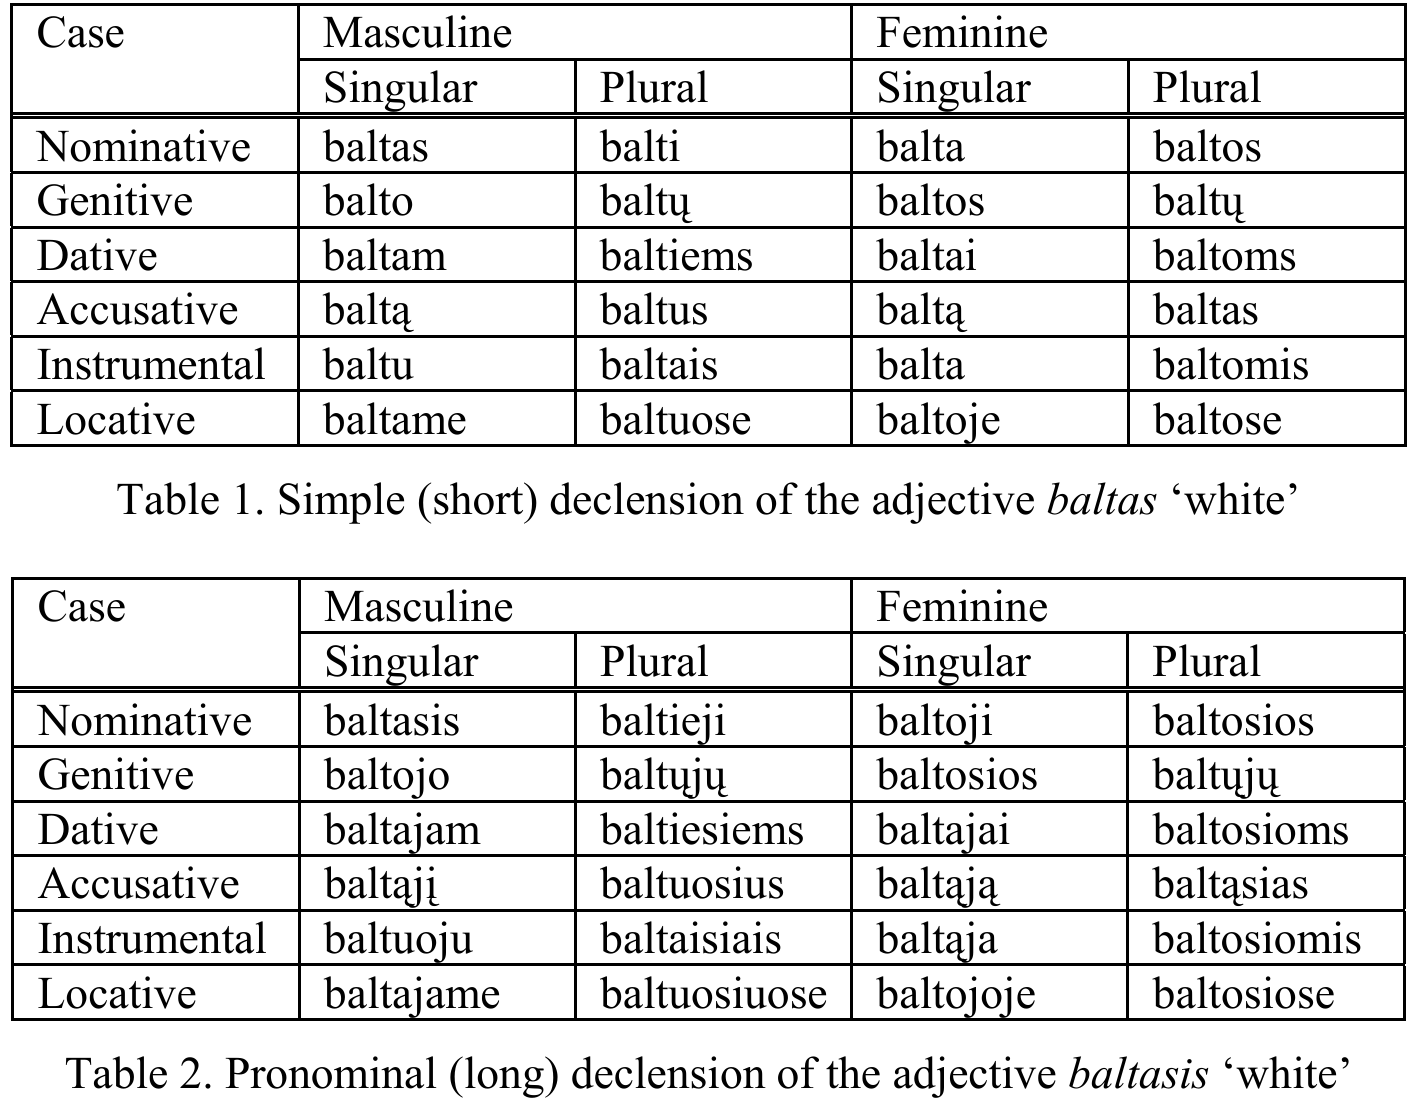
\includegraphics[width=35em]{lit paradigm.png}

\end{frame}

\begin{frame}
    \frametitle{Классифицирующие прилагательные}

    Однако тот же маркер имеют классифицирующие прилагательные, втч. такие, которые вместе с существительным обозначают вид \citep{rutpro2006}

    \pex<class>
        \a \begingl
            \gla formali-oji\ /\ *-a logika//
            \glb формальный-\Def{}.\F{}\ /\ -\F{} логика//
            \glft 'формальная логика'//
        \endgl
        \a \begingl
            \gla baltas*(-is) lokys//
            \glb белый-\Def{} медведь//
            \glft 'белый (полярный) медведь'\trailingcitation{\citep{sereikaite2017}}//
        \endgl
    \xe
    
    \pause    
    Он независим от «настоящего» маркера определенности
    
    \pex<>
        \a \begingl
            \gla gražus baltas-is lokys//
            \glb красивый белый-\Def{} медведь//
            \glft '(a) красивый белый медведь'//
        \endgl
        \a \begingl
            \gla gražus-is baltas-is lokys//
            \glb красивый-\Def{} белый-\Def{} медведь//
            \glft '(the) красивый белый медведь'\trailingcitation{\citep{sereikaite2017}}//
        \endgl
    \xe

\end{frame}


\begin{frame}
    \frametitle{Внутри NP}

    \citep{rutpro2006} о литовском: классифицирующие прилагательные порождаются внутри NP

    Например, они правее других модификаторов

    \pex<lin>
        \a<> \begingl
            \gla Reginos žali-oji arbata//
            \glb Регина.\Gen{} зеленый-\Def{}.\F{} чай//
            \glft 'Регинин зеленый чай'//
        \endgl
        \a<> \begingl
            \gla \ljudge{$^{\#}$}žali-oji Reginos arbata//
            \glb зеленый-\Def.\F{} Регина.\Gen{} чай//
            \glft ожид. 'зеленый Регинин чай'//
        \endgl
    \xe

    в отличие от обычных AP-шных прилагательных

    \pex
        \a<> \begingl
            \gla \ljudge{$^{\#}$}Reginos žali-a suknelė//
            \glb Регина.\Gen{} зеленый-\Def{}.\F{} платье//
            \glft ожид. 'Регинино зеленое платье'//
        \endgl
        \a<> \begingl
            \gla žali-a Reginos suknelė//
            \glb зеленый-\Def.\F{} Регина.\Gen{} платье//
            \glft 'зеленое Регинино платье'//
        \endgl
    \xe
    
\end{frame}

\begin{frame}
    \frametitle{Референция к видам внутри DP}

    Милена Шерейкайте \citep{sereikaite2017}: в каждой (литовской) DP есть оператор $^\cap$.

    Как и $\iota$ в D, он маркируется нулем в отсутствие прилагательного

    \ex<>
        \begingl
            \gla gražus-is baltas-is lokys//
            \glb красивый-\Def{} белый-\Def{} медведь//
            \glft 'красивый полярный медведь'//
        \endgl
    \xe
    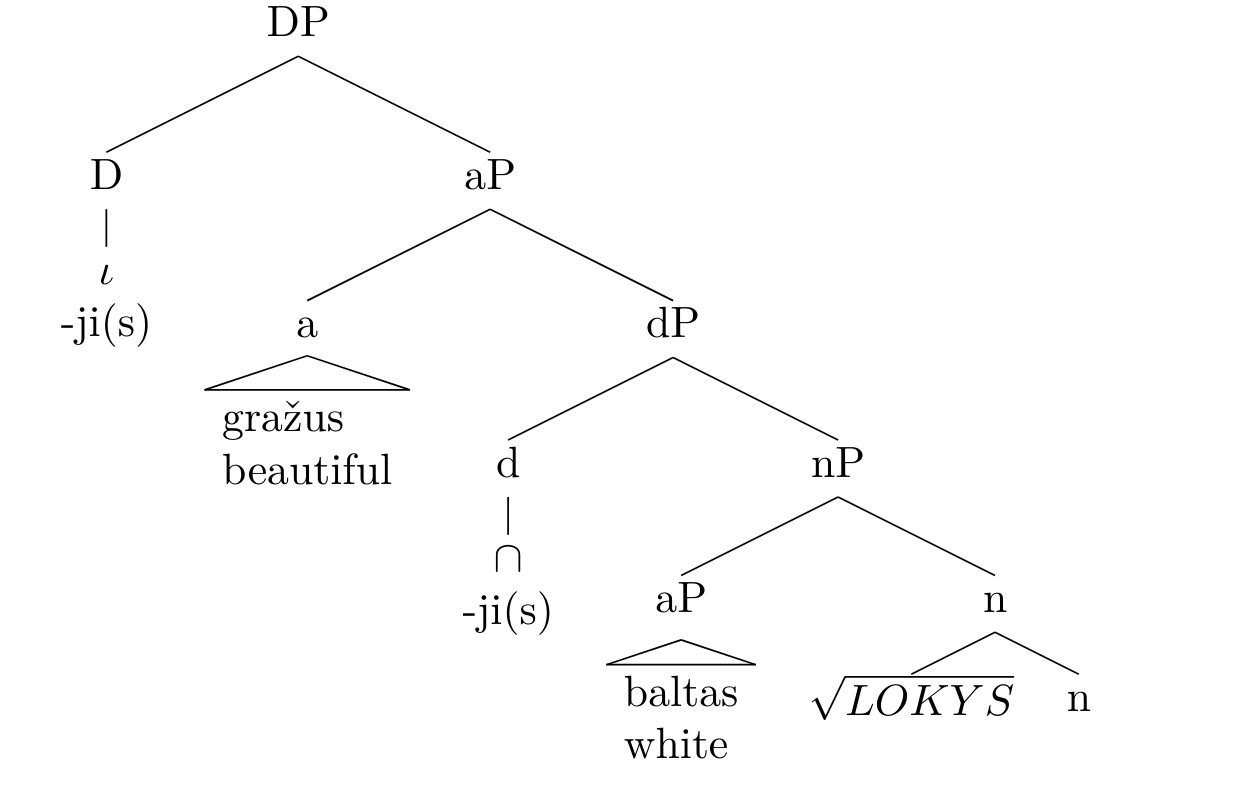
\includegraphics[width=20em]{sereitree.png}

    \pause
    dP типа $e$: необходим еще и оператор $^\cup$ между dP и aP

\end{frame}

\section{Латышский}
\begin{frame}
    \frametitle{Определенность}

    Данные схожи

    \pex<def>
        \a \begingl
            \gla skaist-s lācis//
            \glb красивый-\Nom{} медведь//
            \glft '(a) красивый медведь'//
        \endgl
        \a \begingl
            \gla skaist-ai-s lācis//
            \glb красивый-\Def{}-\Nom{} медведь//
            \glft '(the) красивый медведь'//
        \endgl
        \a \begingl
            \gla balt-*(ai)-s lācis//
            \glb белый-\Def{}-\Nom{} медведь//
            \glft '(a/the) полярный медведь'//
        \endgl
        \a \begingl
            \gla liel-s \judge{/} liel-ai-s balt-ai-s lācis//
            \glb большой-\Nom{} / большой-\Def-\Nom{} белый-\Def-\Nom{} медведь//
            \glft '(a) / (the) большой белый медведь'//
        \endgl
    \xe

\end{frame}

\begin{frame}
    \frametitle{Парадигма}

    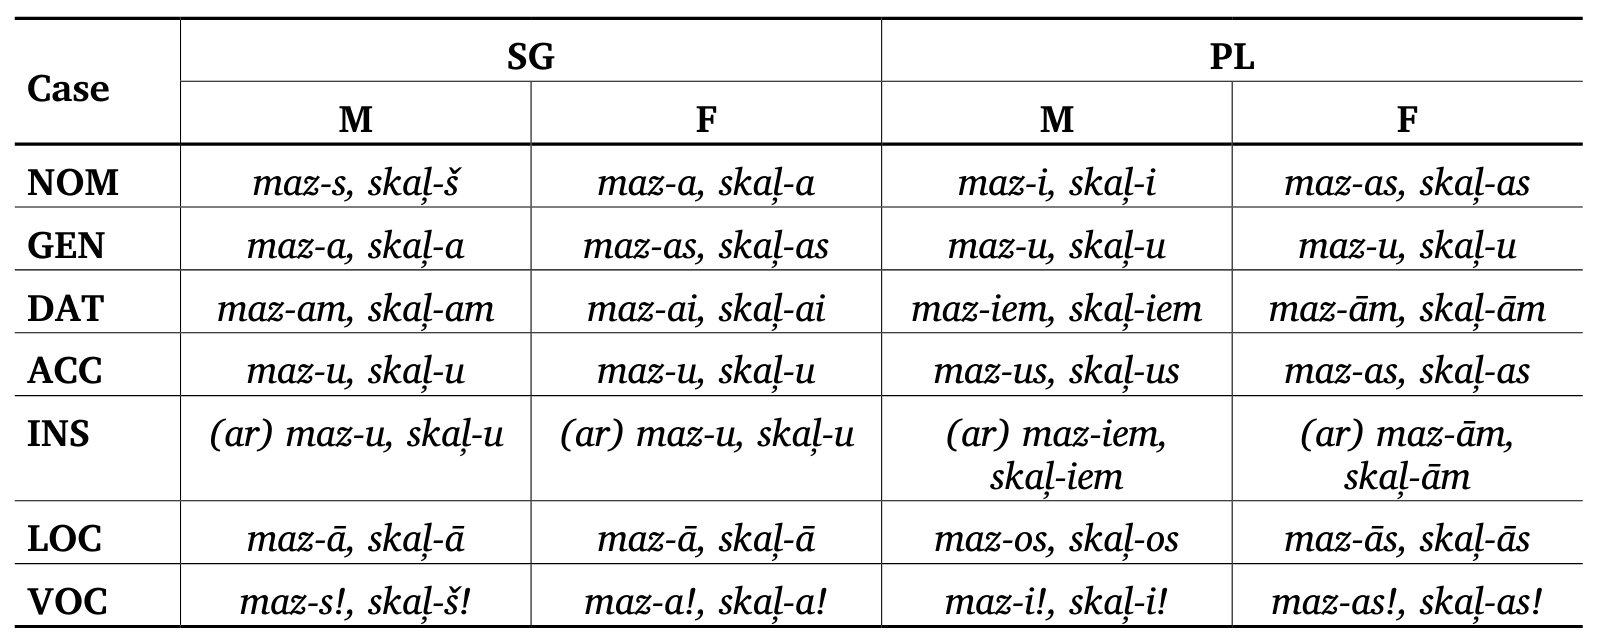
\includegraphics[width=30em]{lat paradigm 1.png}
    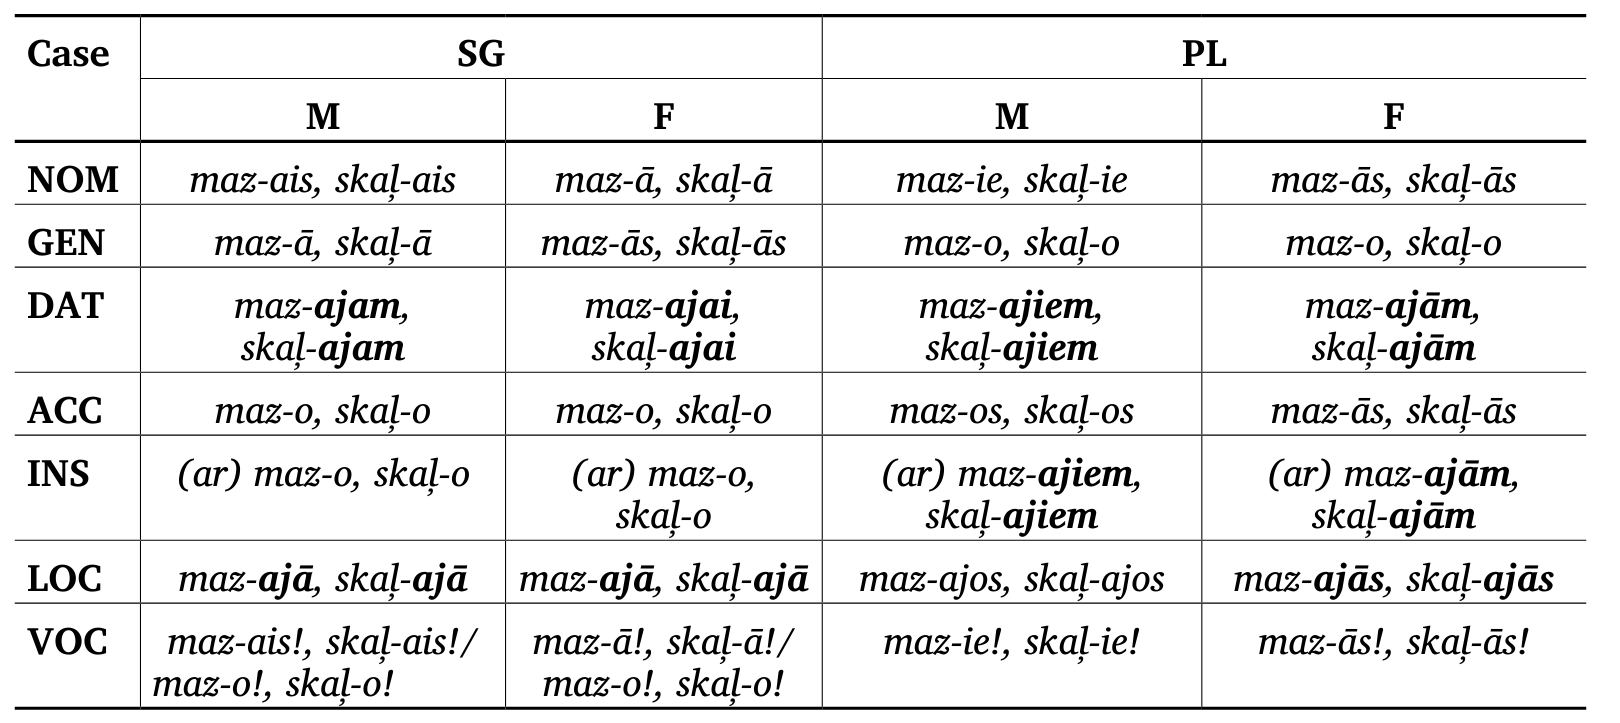
\includegraphics[width=30em]{lat paradigm 2.png}

\end{frame}

\begin{frame}
    \frametitle{Несколько прилагательных}

    Однако в латышском доступно несколько маркеров определенности в ИГ

    \ex<>
        \begingl
            \gla liel-ai-s balt-ai-s kaķis//
            \glb большой-\Def-\Nom{} белый-\Def-\Nom{} кот//
            \glft '(the) большой белый кот'//
        \endgl
    \xe

    \pause

    Более того, определенное прилагательное не может быть левее неопределенного

    \ex<>
        \begingl
            \gla \ljudge*liel-ai-s balt-s kaķis//
            \glb большой-\Def-\Nom{} белый-\Nom{} кот//
            \glft ожид. 'большой белый кот'//
        \endgl
    \xe

\end{frame}

\begin{frame}
    \frametitle{Определенность внутри ИГ}

    Обратный порядок влечет «партитивную» интерпретацию

    \ex<>
        \begingl
            \glpreamble \{Идя по улице, я увидел несколько белых котов. Ко мне подошел\}//
            \gla liel-s balt-ai-s kaķis//
            \glb большой-\Nom{} белый-\Def-\Nom{} кот//
            \glft 'большой белый кот'//
        \endgl
    \xe

    \pause
    Аналогично — под индефинитом
    \ex<>
        \begingl
            \glpreamble \{На столе стоят кружки, большие и маленькие. Я прошу:\}//
            \gla iedod man kād-u liel-o krūzi//
            \glb подай мне какой-нибудь-\Acc{} большой-\Def{}.\Acc{} кружка-\Acc{}//
            \glft 'Подай мне какую-нибудь из больших кружек'//
        \endgl
    \xe

    \pause
    Таким образом, латышская определенность не пресуппонирует уникальность

    И в этом отношении ничем не отличается от видового маркирования

\end{frame}

\begin{frame}[c]
    \frametitle{Партитивная специфичность}

    Латышский \textit{-ai-} маркирует \textbf{партитивную специфичность} [\citealt{enc1991} и др.]

    \ex<>
        $\llbracket ai \rrbracket = \lambda P\lambda x.\ x\le \iota P$
    \xe

    \pause
    
    \onslide<2>{
        \ex<>
            \begingl
                \gla balt-ai-s kaķis//
                \glb белый-\Def-\Nom{} медведь//
                \glft $\lambda y.\ y\le\iota(\lambda x.\ \textsc{белый}(x) \land \textsc{кот}(x))$\\
                истинно для любого индивида, входящего во множество контекстно салиентных котов\footnote{Мы преполагаем, что все имена входят в деривацию неспецифицированными по числу — «массовыми» [\citealt{sauerland2003}; \citealt{scontras2014}; и др.]}//
            \endgl
        \xe
    }

\end{frame}

\begin{frame}
    \frametitle{Вместо понижения}

    Предложение (\nextx) имеет некоторый маркер прямо над NP
    \ex<>
        \begingl
            \gla liel-s balt-ai-s lācis//
            \glb большой-\Nom{} белый-\Def-\Nom{} медведь//
            \glft 'большой полярный медведь'//
        \endgl
    \xe

    \pause
    
    \pex<>
        \a $^\cap P_{\langle s\langle e,t\rangle\rangle} = \lambda s.\ \iota P_s \text{ iff }\lambda s.\ \iota P_s\in K$
        \a $^\cup k = \lambda x.\ x\le k_s$
        \a (игнорируя интенсиональность)\\ $^\cup(^\cap P) = \lambda x.\ x\le \iota P\text{ iff }\iota P\in K$
    \xe

    \ex<>
        $\llbracket ai \rrbracket = \lambda P\lambda x.\ x\le \iota P$
    \xe

    \pause
    Но требование $\iota P\in K$ удовлетворяется per se: внутри NP могут быть только классифицирующие прилагательные

\end{frame}

\begin{frame}
    \frametitle{Определенность и виды}

    \pex
        \a<>\begingl
            \gla liel-s \ljudge{[$_\text{AP}$\ }balt-ai-s @ kaķis\judge{]}//
            \glb большой-\Nom{} белый-\Def-\Nom{} кот//
            \glb $\lambda x.\ \textsc{большой}(x)$ $\lambda x.\ x\le\iota(\lambda x.\ \textsc{белый}(x)$ $\ \land\ \textsc{кот}(x))$//
            \glft 'Неопределенный большой индивид, входящий во множество контекстно салиентных белых котов.'\vspace{1em}//
        \endgl
        \a<> \begingl
            \gla liel-s \ljudge{[$_\text{NP}$\ }balt-ai-s @ lācis\judge{]}//
            \glb большой-\Nom{} белый-\Def-\Nom{} медведь//
            \glb $\lambda x.\ \textsc{большой}(x)$ $\lambda x.\ x\le\iota(\lambda x.\ \textsc{белый\_}$ $\textsc{медведь}(x))$//
            \glft 'Неопределенный большой индивид, входящий во множество полярных медведей.'//
        \endgl
    \xe
    \pause
    
    Почему \textit{baltais lācis} — множество всех белых медведей, а \textit{baltais kaķis} — множество \textbf{контекстно салиентных} белых котов?

    Видимо, контекстная переменная C \citep{fintel1994} адъюнгируется только к высоким прилагательным
\end{frame}

\begin{frame}
    \frametitle{Максимизация}

    Почему определенное прилагательное не может быть над неопределенным?

    \ex<>
        \begingl
            \gla liel-ai-s balt-*(ai)-s kaķis//
            \glb большой-\Def-\Nom{} белый-\Def-\Nom{} кот//
            \glft '(the) большой белый кот'//
        \endgl
    \xe

    \pause
    
    Случай максимизации пресуппозиции \citep{heim1991, copbeav2015}
    \begin{itemize}
        \item[] Сущ. множество контекстно салиентных больших белых котов 
        \item[$\Rightarrow$] сущ. множество контекстно салиентных белых котов 
        \item[$\Rightarrow$] пресуппозиция на balts всегда будет удовлетворяться
    \end{itemize}

\end{frame}

\begin{frame}
    \frametitle{Что еще непонятно}

    Классифицирующих прилагательных может быть несколько — в этом случае маркируется каждое из них

    \ex<>
        \begingl
            \gla liel-ā akademisk-ā vārdnīca//
            \glb большой-\Def.\F{} академический-\Def.\F{} словарь//
            \glft 'Большой академический словарь'//
        \endgl
    \xe

    \citep{sereikaite2017}: конкорд

\end{frame}

\begin{frame}
    \frametitle{Итоги}

    \begin{itemize}
        \item Подобно литовскому, латышский суффикс определенности на прилагательных служит для маркирования видов внутри ИГ
        \item Это значение легко объединяется с базовым значением суффикса — партитивной специфичностью
        \item Таким образом различие видовой и индивидной референции можно представлять синтаксически
        \item Остается актуальным вопрос контекстуальной рестрикции
        \item а также маркирования нескольких Классифицирующих прилагательных
    \end{itemize}

\end{frame}

\begin{frame}
    \frametitle{Библиография}

    {\footnotesize \bibliography{ref.bib}}

\end{frame}
\end{document}
